\documentclass[a4paper,11pt]{article}
\usepackage{graphicx}
\usepackage{float}
\usepackage{subfig}
\usepackage{geometry}
\usepackage{amsmath,amssymb}
\usepackage{amsthm}
\usepackage{bbold}
\usepackage{mathtools}
\usepackage{braket}
\usepackage{booktabs}
\usepackage[table,xcdraw]{xcolor}
\usepackage[utf8]{inputenc}
\usepackage{cite}
\usepackage[english]{babel}
\usepackage{lipsum}
\usepackage{setspace}
%\usepackage{minted}
\usepackage{xcolor}
\newcommand{\R}{\mathbb{R}}
\usepackage{hyperref}
\hypersetup{colorlinks=true,linkcolor=blue}
\geometry{a4paper, top=2.5cm, bottom=2.5cm, left=3cm, right=2.5cm}

\begin{document}
	\author{Catalano Giuseppe, Cerrato Nunzia}
	\title{Numerical Linear Algebra Homework Project 3:\\Eigenvalues and Eigenvectors}
	\date{}
	\maketitle
	
\section*{Problem 1}
\textbf{(1)}
We want to reduce the symmetric matrix $A$
\begin{equation}\label{key}
	A = \begin{bmatrix}
		4 & -1 & -1 & 0 \\
		-1 & 4 & 0 & -1 \\
		-1 & 0 & 4 & -1 \\
		0 & -1 & -1 & 4
	\end{bmatrix} 
\end{equation}
to a tridiagonal form using Housholder similarity transformations. The matrix $A$ can be expressed in the following, compact way:
\begin{equation}
	A =  \left[ 
\begin{array}{c|ccc}
	a_{11}&  & \textbf{x}^T  &  \\
	\hline
	&  &  &  \\
	\textbf{x}&  & \hat{A}_1 &  \\
	&  &  & 
\end{array}\right] .
\end{equation}
Let us define the vector $\textbf{u}_{1}$
\begin{equation}\label{key}
	\textbf{u}_1 = \textbf{x} + \text{sgn}(x_1) \lVert \textbf{x}\rVert_2 \textbf{e}_1
\end{equation}	
% = \begin{bmatrix}
%		-1-\sqrt{2}\\
%		-1\\
%		0
%	\end{bmatrix},
%\end{equation}
thanks to which we can define the matrix $\hat{R}_1$
\begin{equation}\label{key}
	\hat{R}_1 = \mathbb{1}_3 - \frac{2}{\lVert \textbf{u}_1\rVert_2^2} \textbf{u}_1 \textbf{u}_1^T
\end{equation}
and a new matrix $R_1$, as follows:
\begin{equation}\label{key}
	R_1 = \left[ 
	\begin{array}{c|ccc}
		1 &  & \textbf{0}^T  &  \\
		\hline
		&  &  &  \\
		\textbf{0}&  & \hat{R}_1 &  \\
		&  &  & 
	\end{array}\right] .
\end{equation}
We will not explicitely construct the matrix $R_1$, as we know that the product $R_1 A$ will assume the following form:
\begin{equation}\label{key}
	R_1 A= \left[ 
	\begin{array}{c|ccc}
		a_{11} &  & \textbf{x}^T  &  \\
		\hline
		-\text{sgn}(x_1) \lVert \textbf{x}\rVert_2  &  &  &  \\
		0 &  & \hat{R}_1 \hat{A}_1 &  \\
		0 &  &  & 
	\end{array}\right] ,
\end{equation}
where the first column is obtained by constuction and the matrix $\hat{R}_1\hat{A}_1$ can be obtained by considering the matrix $\hat{A}_1$ written by columns as $\hat{A}_1 = \left[ ( \hat{A}_1)_1,( \hat{A}_1)_2,( \hat{A}_1)_3 \right] $. Hence $\hat{R}_1\hat{A}_1 = \left[ ( \hat{R}_1\hat{A}_1)_1,( \hat{R}_1\hat{A}_1)_2,(\hat{R}_1 \hat{A}_1)_3 \right] $, where we know that a singole column can be computed as:
\begin{equation}\label{key}
	( \hat{R}_1\hat{A}_1)_i = (\hat{A}_1)_i - \frac{2}{\lVert \textbf{u}_1\rVert_2^2} \textbf{u}_1 \textbf{u}_1^T(\hat{A}_1)_i .
\end{equation}
By expliciting all the terms, we obatin:
\begin{equation}\label{key}
	R_1 A = \begin{bmatrix}
		4 & -1 & -1 & 0 \\
		\sqrt{2} & -2\sqrt{2} & -2\sqrt{2} & \sqrt{2} \\
		0 & -2\sqrt{2} & 2\sqrt{2} & 0 \\
		0 & -1 & -1 & 4
	\end{bmatrix}.
\end{equation}
Since we want to obtain a tridiagonal matrix, we have to compute the matrix $R_1 A R_1$, namely:
\begin{equation}\label{key}
	R_1 A R_1 = \left[ 
	\begin{array}{c|ccc}
		a_{11} &  \lVert \textbf{x}\rVert_2 &  0 & 0 \\
		\hline
		 \lVert \textbf{x}\rVert_2  &  &  &  \\
		0 &  & \hat{R}_1 \hat{A}_1 \hat{R}_1  &  \\
		0 &  &  & 
	\end{array}\right].
\end{equation}
 Knowing that $\hat{R}_1 \hat{A}_1 \hat{R}_1 = (\hat{R}_1 \hat{A}_1 \hat{R}_1)^T = (\hat{R}_1)^T (\hat{R}_1 \hat{A}_1 )^T =\hat{R}_1 (\hat{R}_1 \hat{A}_1 )^T$, we can apply $\hat{R}_1$ to $(\hat{R}_1 \hat{A}_1 )^T$ by columns:
 \begin{equation}\label{key}
	\left[ \hat{R}_1 \hat{A}_1 \hat{R}_1 \right]_i = 	\left[ (\hat{R}_1 \hat{A}_1 )^T \right]_i  - \frac{2}{\lVert \textbf{u}_1\rVert_2^2} \textbf{u}_1 \textbf{u}_1^T	\left[ (\hat{R}_1 \hat{A}_1 )^T \right]_i ,
\end{equation}
obtaining the following form for the matrix $R_1 A R_1 $:
\begin{equation}\label{key}
		R_1 A R_1 = \left[ \begin{array}{cccc}
		4 & \sqrt{2} & 0 & 0 \\
		\sqrt{2} & 4 & 0 & \sqrt{2} \\
		0 & 0 & 4 & 0 \\
		0 & \sqrt{2} & 0 & 4
	\end{array} \right] .
\end{equation}
By identifying the submatrix $	\hat{R}_1 \hat{A}_1 \hat{R}_1$ as
\begin{equation}\label{key}
	\hat{R}_1 \hat{A}_1 \hat{R}_1 = \left[ \begin{array}{ccc}
		4 & 0 & \sqrt{2} \\
		0 & 4 & 0 \\
		\sqrt{2} & 0 & 4
	\end{array} \right]  =  \left[ \begin{array}{cc}
	(\hat{R}_1 \hat{A}_1 \hat{R}_1)_{11}& \textbf{y}^T \\
	\textbf{y} & \hat{A}_2 
\end{array} \right],
\end{equation}	
we can build the vector $\textbf{u}_2 $ as
\begin{equation}\label{key}
	\textbf{u}_2 = \textbf{y} + \text{sgn}(y_1) \lVert \textbf{y}\rVert_2\textbf{e}_1^{(2)},
\end{equation}	
%\begin{equation}\label{key}
%	 = \sqrt{2} \begin{bmatrix}
%		1\\
%		1
%	\end{bmatrix}
%\end{equation}	
which will allow us to define the matrix $\hat{R}_2$
\begin{equation}\label{key}
	\hat{R}_2 = \mathbb{1}_2 - \frac{2}{\lVert \textbf{u}_2\rVert_2^2} \textbf{u}_2 \textbf{u}_2^T.
\end{equation}
Using the same logic, we obtain the i-th column of the matrix $\hat{R}_2\hat{A}_2$, namely:
\begin{equation}\label{key}
	( \hat{R}_2\hat{A}_2)_i = (\hat{A}_2)_i - \frac{2}{\lVert \textbf{u}_2\rVert_2^2} \textbf{u}_2 \textbf{u}_2^T(\hat{A}_2)_i,
\end{equation}
and, by expliciting all the terms we obtain:
\begin{equation}\label{key}
	\hat{R}_2 \hat{A}_2 = \left[ \begin{array}{cc}
		0 & -4 \\
		-4 & 0
	\end{array}\right].
\end{equation}
As before, we can compute $\hat{R}_2 \hat{A}_2 \hat{R}_2$ by columns, and the final form of the matrix will be:
\begin{equation}\label{key}
	R_2R_1AR_1R_2 =\begin{bmatrix}
		4& \sqrt{2} & 0  &  0\\
		\sqrt{2}&4 & -\sqrt{2} & 0\\
		0 & -\sqrt{2} & 4  & 0 \\
		0 & 0 & 0 & 4
	\end{bmatrix}.
\end{equation}
As we can see, we have reduced the initial matrix $A$ to tridiagonal form.\\

\noindent \textbf{(2)} In the following we report the script where we implement the QR diagonalization of a matrix $A$, defined as:
\begin{equation}
	A = \begin{bmatrix}
		4 & 3 & 2 & 1 \\
		3 & 4 & 3 & 2 \\
		2 & 3 & 4 & 3 \\
		1 & 2 & 3 & 4
	\end{bmatrix}
\end{equation}.

*** INSERIRE CODICE ***\\

\noindent Here we report the intermediate $A_k$ matrices for $k = 1, 10, 15, 15$ and the final one with $k = 21$:

** inserire matrici **\\

\noindent We can observe the decreasing of the off-diagonal entries and the convergence of the diagonal terms to the eigenvalues computed using the function np.linalg.eigvals, which we consider as exact. The maximum absolute error on the eigenvalues is of the order of $10^{-8}$.\\

\noindent In the following script we implement the QR diagonalization of the matrix $A$ using the Rayleigh quotient shift and deflation. \\

*** inserire codice ***\\

\begin{figure}[H]
	\centering
	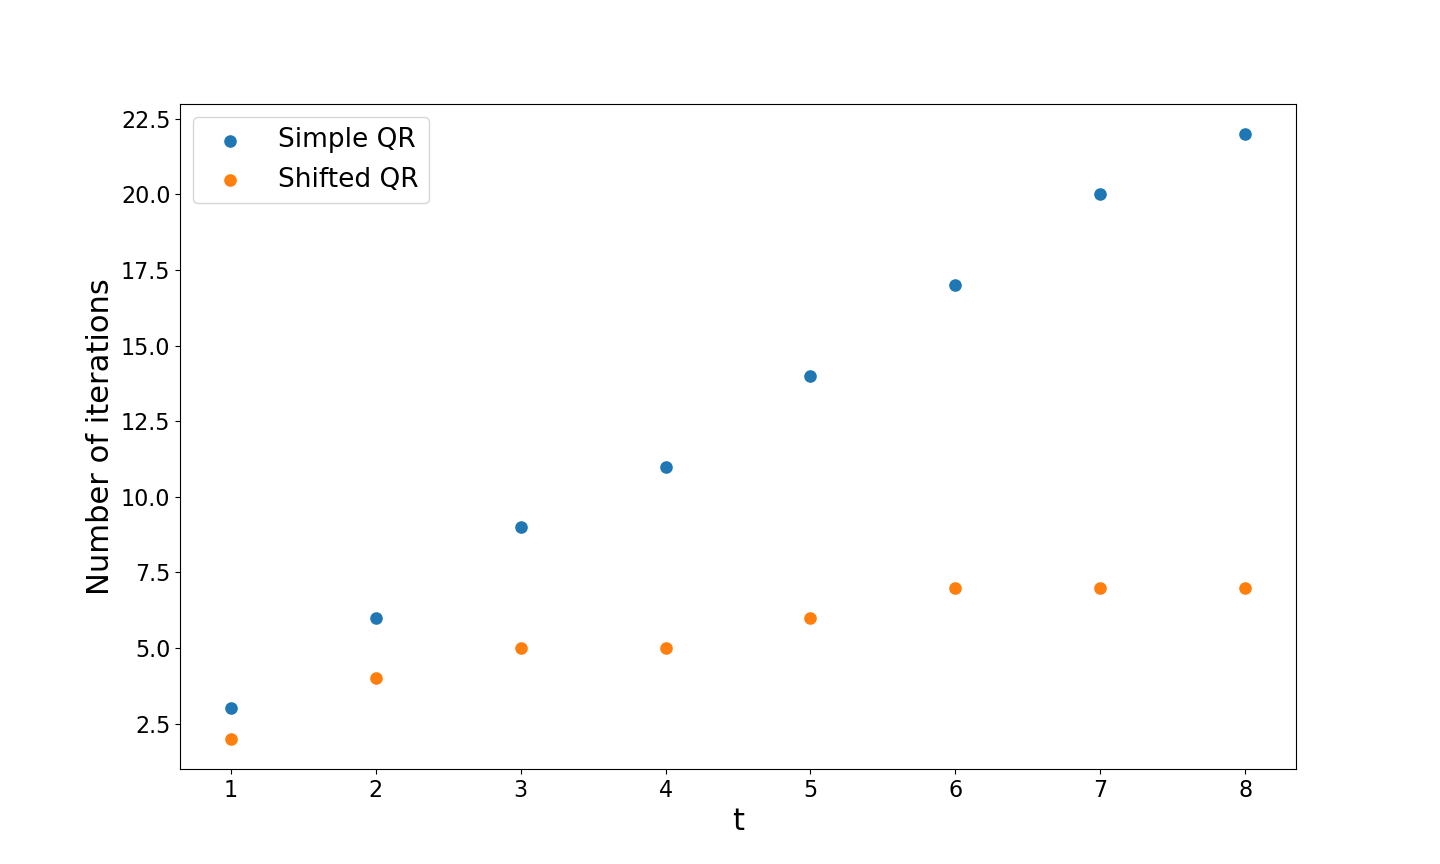
\includegraphics[scale=0.40]{Plot/Plot_QR_Standard_Rayleigh.png}
	\caption{Number of iteration needed to achieve a maximum absolute error less than $10^{-t}$ on the eigenvalues computed by using standard and shifted QR iteration algorithm.}
	\label{Fig:Num_iter_with_t}
\end{figure}

\noindent As we see from Fig. \ref{Fig:Num_iter_with_t}  the number of iteration required to achieve a maximum absolute error less than $10^{-t}$ on eigenvalues appears to grow linearly with $t$ in the case of the simple QR iteration algorithm. On the other hand, in the case of the shifter QR iteration algorithm, implemented by using the Rayleigh shift, the same error appears to grow sublinearly with $t$, meaning that this last algorithm reaches the required tolerance with a less number of iterations, thus being faster.

	
\section*{Problem 2}	
Here we consider approximations to the eigenvalues and eigenfunctions of the one-dimensional Laplace operator 
$L[u] := - \frac{d^2 u }{dx^2}$ on the unit interval $[0,1]$ with boundary conditions $u(0) = u(1) = 0$. A scalar $\lambda$ is said to be an eigenvalue of $L$ (with homogeneous Dirichlet boundary conditions) if there exists a twice-differentiable function $u : [0, 1] \rightarrow \R$, not identically zero in $[0, 1]$, such that
\begin{equation}\label{eq: continuous differential eigenproblem}
	-u''(x) = \lambda u(x) \text{ on } [0,1] \text{ with } u(0) = u(1) = 0.
\end{equation}
In this case $u$ is said to be an \textit{eigenfunction} of $L$ corresponding to the eigenvalue $\lambda$. Obviously, eigenfunctions are defined up to a nonzero scalar multiple.
The eigenvalues and eigenfunctions of $L$ are easily found to be $\lambda_j = j^2\pi^2$ and $u_j(x) = \alpha \sin(j\pi x)$ for any nonzero constant $\alpha$, which we can take to be $1$. Here $j$ is a positive integer; hence, the operator $L$ has an infinite set of (mutually orthogonal) eigenfunctions $\{u_j\}_{j=1}^\infty $ corresponding to the discrete spectrum of eigenvalues ${\lambda_j}_{j=1}^\infty $. Note that $0 < \lambda_1 < \lambda_2 < \dots < \lambda_j \rightarrow \infty$ as $j \rightarrow \infty$. Also, each eigenvalue is simple in the sense that (up to a scalar multiple) there is a unique eigenfunction corresponding to it. Approximations to the eigenvalues and eigenfunctions can be obtained by discretizing the interval $[0, 1]$ bymeansof $N+2$ evenly spaced points: $x_i =ih \text{ where } i=0,1,...,N+1 \text{ and } h=1/(N+1)$. The second derivative operator can then be approximated by centered finite differences:

\begin{equation}
	-\frac{d^2u}{dx^2}(x_i) \approx \frac{-u(x_{i-1} + 2 u(x_i)  -2 u(x_{i+1}) )}{h^2}
\end{equation}
and therefore the continuous (differential) eigenproblem \eqref{eq: continuous differential eigenproblem} can be approximated by the discrete (algebraic) eigenvalue problem 

\begin{equation}\label{key}
	h^{-2} T_N \textbf{u} = \lambda \textbf{u}
\end{equation}
where we have set

\begin{equation}\label{key}
	T_N = \begin{bmatrix}
		2 & -1 &  & 0 \\
		-1 & \ddots  & \ddots  &  \\
		& \ddots & \ddots & -1 \\
		0 &  & -1 & 2
	\end{bmatrix}, \text{ and } \textbf{u} = \begin{bmatrix}
		u_1\\
		u_2\\
		\vdots\\
		u_N
	\end{bmatrix} 
\end{equation}
with $u_i := u(x_i)$. It can be shown that the $N \times N$ matrix $T_N$ has eigenvalues $\mu_j = 2(1- \cos \frac{\pi j }{N+1})$ for $j = 1, \dots, N$, corresponding to the eigenvectors $\textbf{u}_j$, where $\textbf{u}_j(k) = \sqrt{\frac{2}{N+1}} \sin( \frac{j k \pi}{N+1} $) is the $kth$ entry in $\textbf{u}_j$. Notice that the eigenvectors $\textbf{u}_j$ are normalized with respect to the 2-norm: $\textbf{u}^T_j \textbf{u}_j = 1$. Also notice that the eigenvalues of $T_N$ lie in the interval $(0, 4)$. Hence, the eigenvalues of $h^{-2} T_N$ lie in the interval $(0, 4(N + 1)2 )$.\\


\noindent \textbf{(1)} Since we are considering $j\ll N$ and $N\gg1$ we can identify the Taylor expansion of $\cos x$ with $x = \frac{\pi j }{N+1}$:
\begin{equation}
	\cos \frac{\pi j }{N+1} = \cos \pi j h = 1 - \frac{1}{2} \pi^2 j^2 h^2 + O(h^4),
\end{equation}
that leads us to approximate the smallest eigenvalues of $2h^{-2} T_N$ as follows:
\begin{equation}\label{key}
	2h^{-2} (1- \cos \frac{\pi j }{N+1} ) = 2h^{-2} (1- 1 + \frac{1}{2} \pi^2 j^2 h^2 + O(h^4)) = \pi^2 j^2  + O(h^2) \simeq \pi^2 j^2,
\end{equation}
where we used that $h=1/N+1$.\\
\noindent For the largest eigenvalue of $T_N$, we have that $j = N$, therefore we can not truncate anymore the taylor expansion of the cosine if we want a good approximation. We can compute the $N-th$ eigenvalue of $T_N$ in the limit of $N\gg 1$:
\begin{equation}\label{key}
	\mu_N = 2(1-\cos\pi  \frac{N}{N+1})  =2(1-\cos (\pi -\pi h) )) = 2(1+cos\pi h) = 4 - \pi^2 h^2 + O(h^4)
\end{equation}
Therefore, we have
\begin{equation}\label{key}
	h^{-2} \mu_N = 4(N+1)^2 - \pi^2 + O(h^2)
\end{equation}
that is not a good approximation of $\lambda_N = \pi^2 N^2$ 

\noindent \textbf{(2)} We want to compare the eigenvectors $\textbf{u}_j$ of $T_N$ with the eigenfunctions of $L$, up to the normalization constant, that we will set to $1$ for both. If we recall that $x_k = k h\ \forall k = 1,\dots, N$ we can observe that the $k-th$ component of the eigenvector $\textbf{u}_j$ is equal to the $j-th$ eigenfunction $u_j(x)$ computed in corrispondence of the value $x=x_k$:
\begin{equation}
	u_j(x_k) = \sin(j \pi x_k) = \sin ( j \pi k h ) = \sin\left( \frac{j \pi k}{N+1}\right)  = \textbf{u}_j(k).
\end{equation}

\noindent \textbf{(3)}  Now we compute the spectral condition number of $T_N$ in the limit of $N\gg 1$. We recall that the eigenvalues of $T_N$ are
\begin{equation}\label{key}
	\mu_j = 2\left( 1-\cos \frac{\pi j}{N+1}\right) = 2\left( 1-\cos \pi j h\right)
\end{equation}
\begin{equation}
	\begin{split}
		h^{-2}\mu_1 &= h^{-2} 2 \left(  1-1 +\frac{1}{2} \pi^2 h^2 - \frac{1}{4!} \pi^4 h^4 + O(h^6)\right) \\
		& = \pi^2 -\frac{1}{12} \pi^4 h^2 + O(h^4)
	\end{split}
\end{equation}

\begin{equation}
	\begin{split}
		h^-2\mu_N &= h^{-2}2(1+cos(\pi h))\\
		&=2h^{-2} \left( 1 + 1 -\frac{1}{2} \pi^2 h^2 + \frac{1}{4!} \pi^4 h^4 + O(h^6)\right) \\
		&= 4 h^{-2} - \pi^2 +\frac{1}{12} \pi^4 h^2 + O(h^4)
	\end{split}
\end{equation}

\begin{equation}
	\begin{split}
		k_2(T_N) &= \frac{h^{-2}\mu_N}{h^{-2}\mu_1} = \frac{4 h^{-2} - \pi^2 +\frac{1}{12} \pi^4 h^2 + O(h^4)}{\pi^2(1 -\frac{1}{12} \pi^2 h^2 + O(h^4))}\\
		&= \frac{4 h^{-2}}{\pi^2} -1 + \frac{4 h^{-2}}{\pi^2} \frac{\pi^2 h^2}{12} +O(h^2)\\
		&=\frac{4}{\pi^2}(N+1)^2 - \frac{2}{3} + O(N^{-2})
	\end{split}
\end{equation}


\end{document}